% =====================================================================
%  Human-in-the-Loop Robot Learning on the FFW SG2
%  System Manual
%
%  Compile: pdflatex (twice, for cross-references), or upload to Overleaf.
%  Colour policy: body text, tables and callouts are monochrome and print
%  correctly in greyscale. Colour is used only in the architecture figures
%  and in code listings, where it carries information rather than decoration.
%
%  Figure placeholders use \placeholder{file}{description}{height}.
%  Replace with \includegraphics when the image is available.
%
%  Two compilation notes, both of which produced blank pages during drafting:
%    - \resizebox{\textwidth}{!} constrains width only. A picture taller than
%      the text block overflows silently. adjustbox with max totalheight
%      constrains both dimensions.
%    - Display math is not permitted inside a TikZ node. The callout
%      environments are TikZ nodes.
% =====================================================================
\documentclass[11pt,a4paper]{article}

\usepackage[margin=2.3cm]{geometry}
\usepackage{pdflscape}
\usepackage{adjustbox}
\usepackage{tikz}
\usepackage{graphicx}
\usepackage{float}
\floatplacement{figure}{H}
\usepackage{longtable}
\usepackage{booktabs}
\usepackage{array}
\usepackage{enumitem}
\usepackage{listings}
\usepackage{xcolor}
\usepackage{fancyhdr}
\usepackage{titlesec}
\usepackage[hidelinks]{hyperref}
\usetikzlibrary{positioning,arrows.meta,fit,backgrounds,calc}

% ---------------- palette (figures and listings only) ----------------
% Deliberately not used in body text or tables, which remain monochrome.
\definecolor{figHuman}{RGB}{170,45,45}     % human commands the arms
\definecolor{figAuto}{RGB}{30,95,175}      % policy commands the arms
\definecolor{figWorker}{RGB}{228,240,252}
\definecolor{figPolicy}{RGB}{235,229,250}
\definecolor{figCyclo}{RGB}{253,240,222}
\definecolor{figUI}{RGB}{229,247,232}
\definecolor{figStore}{RGB}{240,240,240}
\definecolor{figFlag}{RGB}{253,228,228}
\definecolor{lstKey}{RGB}{20,80,160}
\definecolor{lstCom}{RGB}{100,120,100}
\definecolor{lstStr}{RGB}{150,60,20}
\definecolor{lstBg}{RGB}{249,249,249}

% ---------------- typography ----------------
\linespread{1.04}
\setlength{\parskip}{0.6em}
\setlength{\parindent}{0pt}
\setlist{itemsep=0.25em,parsep=0em,topsep=0.35em}

\titleformat{\section}{\large\bfseries}{\thesection}{0.8em}{}
\titleformat{\subsection}{\normalsize\bfseries}{\thesubsection}{0.8em}{}
\titlespacing*{\section}{0pt}{2.4ex plus 1ex minus .2ex}{1.4ex plus .2ex}

\pagestyle{fancy}
\fancyhf{}
\fancyhead[L]{\footnotesize Human-in-the-Loop Robot Learning --- FFW SG2}
\fancyhead[R]{\footnotesize\thepage}
\renewcommand{\headrulewidth}{0.4pt}

% ---------------- listings ----------------
\lstset{
  basicstyle=\ttfamily\footnotesize,
  keywordstyle=\color{lstKey}\bfseries,
  commentstyle=\color{lstCom}\itshape,
  stringstyle=\color{lstStr},
  backgroundcolor=\color{lstBg},
  breaklines=true,
  showstringspaces=false,
  frame=single,
  framesep=5pt,
  xleftmargin=0pt,
  columns=fullflexible,
  keepspaces=true,
  captionpos=b,
  abovecaptionskip=4pt,
}
\lstdefinestyle{sh}{language=bash}
\lstdefinestyle{py}{language=Python}
\lstdefinestyle{yml}{
  morekeywords={observation,images,state,action,recording,extra_topics,topic,
                rotation_deg,upper_body,mobile,arm_left,arm_right,head,lift},
  morecomment=[l]{\#}}

% ---------------- callouts (ruled, unfilled) ----------------
\newcommand{\callout}[2]{%
  \par\medskip\noindent
  \begin{tikzpicture}
    \node[draw=black,line width=#1,inner sep=3mm,
          text width=\dimexpr\linewidth-8mm\relax,align=left] {#2};
  \end{tikzpicture}\par\medskip}
\newcommand{\caution}[1]{\callout{1pt}{#1}}
\newcommand{\remark}[1]{\callout{0.4pt}{#1}}

% ---------------- figure placeholder ----------------
\newcommand{\placeholder}[3]{%
  \begin{center}
  \begin{tikzpicture}
    \node[draw=black!55,dashed,rounded corners=1pt,
          minimum height=#3,minimum width=0.88\linewidth,align=center,
          font=\footnotesize,text width=0.82\linewidth]
      {\textsc{figure placeholder}\\[1.2mm]
       \texttt{\detokenize{#1}}\\[1.2mm] #2};
  \end{tikzpicture}
  \end{center}}

% =====================================================================
\begin{document}

\begin{titlepage}
\centering
\vspace*{3.2cm}
{\Large\scshape Human-in-the-Loop Robot Learning}\\[3mm]
\rule{9cm}{0.5pt}\\[4mm]
{\LARGE\bfseries System Manual}\\[10mm]
{\large FFW SG2 follower \quad A2 leader}\\[24mm]

\begin{minipage}{12cm}
\small
\textsc{Scope.} The architecture of the teleoperation, policy and orchestration
subsystems; the procedure for conducting an HG-DAgger session; the contents of
the resulting dataset; and the training and verification procedures that follow
from it.

\end{minipage}

\vfill
{\small ROBOTIS \quad 31 August 2026}
\end{titlepage}

\tableofcontents
\thispagestyle{empty}
\newpage
\setcounter{page}{1}

% =====================================================================
\section{System overview}

The system comprises three containers and a browser client.

\begin{center}
\small
\begin{tabular}{@{}lp{10.2cm}@{}}
\toprule
\textbf{Component} & \textbf{Responsibility}\\
\midrule
\texttt{ai\_worker}          & Hardware. Leader and follower arms, head, lift, swerve base, four cameras.\\
\texttt{groot\_server}       & Policy inference. GR00T-N1.7 on a TensorRT DiT backend.\\
\texttt{cyclo\_intelligence} & Orchestration, recording, dataset conversion, external interfaces.\\
Browser                      & Operator interface for policy control, intervention and labelling.\\
\bottomrule
\end{tabular}
\end{center}

The policy commands sixteen dimensions, corresponding to the two arms. The head,
lift and mobile base are never commanded by the policy ($22-6=16$).

\subsection{Shared command topic}

The teleoperation node and the policy publish to the same arm-command topic (thus the SG2 robot).
There is no separate policy channel. There are two consequences that follow:

\begin{enumerate}
\item The recorded \texttt{action} column is valid irrespective of which agent
      was driving, since both write to the topic that is recorded.
\item Mutual exclusion must be enforced externally. A latched flag (T14)
      suppresses the leader chain while the policy is active.
\end{enumerate}

\subsection{Session structure}

The policy executes the task autonomously. When its behaviour is incorrect the
operator suspends it, corrects the motion by teleoperation, and returns control.
The corrected frames constitute the training signal. The purpose of the
surrounding system is to make this exchange safe and to record which frames
originated from the operator.

\begin{figure}[H]
    \centering
    \includegraphics[width=0.75\linewidth]{\detokenize{figs/session overview.png}}
    \caption{Work cell during a session: follower arms engaged on the task, leader arms held by the operator, operator UI.}
    \label{fig:cell}
\end{figure}

% =====================================================================
\newpage
\section{Software Requirements}
\label{sec:obtain}

\subsection{Repositories}

\begin{center}
\small
\begin{tabular}{@{}lll@{}}
\toprule
\textbf{Repository} & \textbf{Branch} & \textbf{Contents}\\
\midrule
\texttt{da-dawit/aiw\_backup}                & \texttt{feature-a2} & Robot-side packages; for a2 leader\\
\texttt{da-dawit/cyclo\_intelligence\_backup} & \texttt{main}       & Orchestration, recording, conversion\\
\texttt{da-dawit/hg-dagger}                  & \texttt{main}       & Training, evaluation and dataset tooling\\
\bottomrule
\end{tabular}
\end{center}

The first two are private; SSH Keys.

\begin{lstlisting}[style=sh]
git clone git@github.com:da-dawit/aiw_backup.git
git clone git@github.com:da-dawit/cyclo_intelligence_backup.git
git clone git@github.com:da-dawit/hg-dagger.git
\end{lstlisting}

\texttt{hg-dagger} contains the scripts referenced throughout
Sections~\ref{sec:train} to~\ref{sec:verify}:

\begin{center}
\small
\begin{tabular}{@{}ll@{}}
\toprule
\textbf{Path} & \textbf{Purpose}\\
\midrule
\texttt{scripts/verify\_dataset.py}      & Dataset validation gate\\
\texttt{scripts/fix\_dagger\_dataset.py} & Repair a converted online-RL dataset\\
\texttt{scripts/split\_dagger.py}        & Partition by intervention label\\
\texttt{configs/export\_dagger\_split.py}& Write the partition as LeRobot datasets\\
\texttt{configs/06\_train\_dagger.sh}    & HG-DAgger training launcher\\
\texttt{scripts/checkpoint\_sweep.py}    & Held-out error per checkpoint\\
\texttt{scripts/rollout3d.py}            & Cartesian rollout evaluation\\
\texttt{scripts/attn\_map.py}            & Attention diagnostics\\
\texttt{scripts/crop\_stats.py}          & Motion energy and detail per crop region\\
\texttt{configs/roi\_hybrid.json}        & Per-camera crop specification\\
\texttt{configs/crop\_to\_square.patch}  & Required patch to Isaac-GR00T\\
\bottomrule
\end{tabular}
\end{center}

\subsection{Branch selection}

\texttt{aiw\_backup} carries two branches. The default is
\texttt{ai\_worker-wip}; the work described in this manual is on
\texttt{feature-a2}, which is thirteen commits ahead of it. A plain clone
therefore checks out the wrong branch.

\begin{lstlisting}[style=sh]
cd aiw_backup
git checkout feature-a2
\end{lstlisting}

\caution{A branch named \texttt{feature-a2} may already exist in a working copy
obtained from a different source. The name does not imply the same history. If a
local \texttt{feature-a2} is already present, do not assume it corresponds to
the branch described here; follow Section~\ref{sec:existing}.}

\subsection{Working copies that already contain a \texttt{feature-a2}}
\label{sec:existing}

Add this repository as an additional remote rather than overwriting the existing
branch. Nothing is lost and the two histories can be compared directly.

\begin{lstlisting}[style=sh]
cd <existing working copy>
git remote add backup git@github.com:da-dawit/aiw_backup.git
git fetch backup

# What does this branch contain that the local one does not?
git log --oneline feature-a2..backup/feature-a2

# Documentation differences only
git diff --stat feature-a2 backup/feature-a2 -- tmp_readmes/
\end{lstlisting}

Check out the fetched branch under a distinct name, leaving the existing branch
untouched:

\begin{lstlisting}[style=sh]
git checkout -b feature-a2-backup backup/feature-a2
\end{lstlisting}

% =====================================================================
\newpage
\section{Installing the training environment}
\label{sec:install}

Training is performed off the robot, on a machine with two or more GPUs of at
least 40\,GB each. The model is loaded in FP32 during training, so the
requirement is memory rather than throughput.

\subsection{Memory requirement}

\begin{center}
\small
\begin{tabular}{@{}lr@{}}
\toprule
\textbf{Component} & \textbf{Memory}\\
\midrule
Parameters, FP32              & 12.6\,GB\\
Gradients, FP32               & 6.5\,GB\\
Optimiser state, FP32         & 13.0\,GB\\
\midrule
Total before activations      & 32.1\,GB\\
\bottomrule
\end{tabular}
\end{center}

\subsection{Procedure}

\begin{lstlisting}[style=sh]
# 1. Python environment. The project requires Python 3.10 exactly; the
#    dataclass definitions do not parse under 3.11 or later.
curl -LsSf https://astral.sh/uv/install.sh | sh
export PATH="$HOME/.local/bin:$PATH"

# 2. Isaac-GR00T, ROBOTIS fork
git clone https://github.com/ROBOTIS-GIT/Isaac-GR00T-n1.7.git Isaac-GR00T
cd Isaac-GR00T && git checkout e81d02b
uv sync --frozen

# 3. Required patches. Neither is present in a fresh clone.
git apply <hg-dagger>/configs/crop_to_square.patch
git apply <hg-dagger>/configs/mixture_ratio.patch

# 4. Modality configuration
cp <hg-dagger>/configs/ffw_sg2_rev1_16d_config.py \
   examples/CYCLO/ffw_sg2_rev1/

# 5. Hugging Face authentication. The backbone is a gated repository, and
#    the token must be present in the training environment, not only in the
#    login shell: torchrun spawns child processes that do not inherit it.
export HF_TOKEN=<token>
uv run huggingface-cli login --token $HF_TOKEN
\end{lstlisting}

\caution{The two patches are required and are verified by the launcher before
training begins. Without \texttt{crop\_to\_square.patch} every camera is
letterboxed, which differs from the configuration the base checkpoint was
trained under. Without \texttt{mixture\_ratio.patch} the \texttt{path@ratio}
syntax is not parsed, all datasets are collapsed into one specification.}
\subsection{The base policy}
\label{sec:base}

This manual covers the HG-DAgger iteration. It begins from a policy that already
performs the task well enough to be worth correcting and improves it from
operator corrections. Producing that policy is separate work, behaviour cloning
on teleoperated demonstrations, and is not described here.

The reference base policy is checkpoint 30{,}000 of a sixteen-dimension run over
31 screwing demonstrations. Download it, or an equivalent of your own, before
starting.

\begin{lstlisting}[style=sh]
huggingface-cli download dawity/groot_screwing35 \
    --include "<base-checkpoint>/*" --local-dir runs/16d_30k/
\end{lstlisting}

\caution{The base policy must have been trained under the image preparation of
Section~\ref{sec:crop} and the same sixteen declared dimensions. The
continuation inherits both. A base trained under different framing, or over a
different modality slice, cannot be warm-started from: the inputs it was fitted
to are not the inputs it would now receive.}

% =====================================================================
\section{Architecture}

The two diagrams overleaf present the runtime control path and the data path
respectively. Edge labels refer to the identifiers defined in
Section~\ref{sec:legend}.

\begin{center}
\small
\begin{tabular}{@{}ll@{}}
\toprule
\textbf{Line} & \textbf{Meaning}\\
\midrule
\textcolor{red}{Red solid}      & Human commands the arms\\
\textcolor{blue}{Blue dashed}   & Policy commands the arms\\
\textcolor{black}{Black solid}  & Status, feedback and control plane\\
\bottomrule
\end{tabular}
\end{center}

% ---------------------------------------------------------------
\begin{landscape}
\thispagestyle{empty}
\vspace*{\fill}
\begin{figure}[H]
\centering
\makebox[\linewidth][c]{\includegraphics[width=1.05\linewidth,height=0.76\textheight,keepaspectratio]{figs/ai_worker.png}}
\caption{Runtime control path. Which agent is driving the arms at each instant,
and the flags that arbitrate between them. Edge labels are the identifiers
listed in Section~\ref{sec:legend}.}
\label{fig:archcontrol}
\end{figure}
\vspace*{\fill}
\end{landscape}

% ---------------------------------------------------------------
\begin{landscape}
\thispagestyle{empty}
\vspace*{\fill}
\begin{figure}[H]
\centering
\makebox[\linewidth][c]{\includegraphics[width=0.85\linewidth,height=0.76\textheight,keepaspectratio]{\detokenize{figs/ai_worker record.png}}}
\caption{Data path. Recording, conversion, and the point at which the
intervention label is attached to each frame.}
\label{fig:archdata}
\end{figure}
\vspace*{\fill}
\end{landscape}

% =====================================================================
\newpage
\section{Conducting a session}

\subsection{Bring-up}
\label{sec:bringup}

The follower is started first, then the leader, then the bridge. The bridge
subscribes to topics created by the preceding two.

\begin{lstlisting}[style=sh]
ros2 launch ffw_bringup ffw_sg2_follower_ai.launch.py
ros2 launch ffw_bringup ffw_a2_leader_ai.launch.py
python3 leader_bridge.py
\end{lstlisting}

The leader and follower \textbf{may both remain active for the duration of a session.}
They do not contend, because T14 suppresses the leader chain while the policy is
driving. Contention between the two indicates that T14 is not being received.

\begin{figure}[H]
    \centering
    \includegraphics[width=0.75\linewidth]{figs/leader_controls.png}
    \caption{A2 leader, tact switch on each handle, and the joystick whose downward drag suspends and resumes the policy. These are the only two controls used during a session.}
\end{figure}

\subsection{Intervention procedure}
\label{sec:loop}

\begin{figure} [H]
    \centering
    \includegraphics[width=0.8\linewidth]{figs/overall_ui.png}
    \caption{Operator UI Page in Cyclo Intelligence.}
    \label{fig:ui}
\end{figure}

The following assumes the policy is executing.

\begin{enumerate}
\item Drag the joystick downward and hold for one second. The policy suspends.
\item Press the tact switch for the arm to be corrected. That arm engages.
\item Press the tact switch again. The arm disengages and the gripper retains
      its teleoperated value.
\item Drag the joystick downward and hold for one second. The policy resumes.
\end{enumerate}

\begin{figure}[H]
\centering
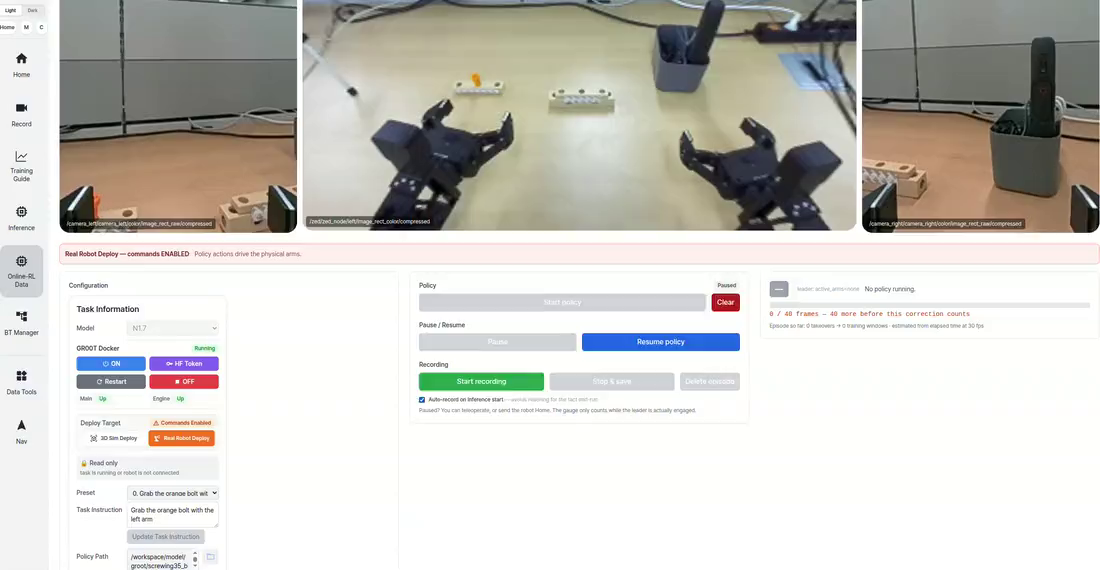
\includegraphics[width=\linewidth]{figs/ui_state_ready.png}
\caption{Before the policy is started. The status panel reads \textsc{no policy
running}, the phase chip reads \textsc{paused}, and \emph{Start policy} is the
available control. The deploy banner already reads \textsc{commands enabled},
which is a property of the connection and not of the policy: nothing is driving
the arms yet.}
\label{fig:uiready}
\end{figure}

\begin{figure}[H]
\centering
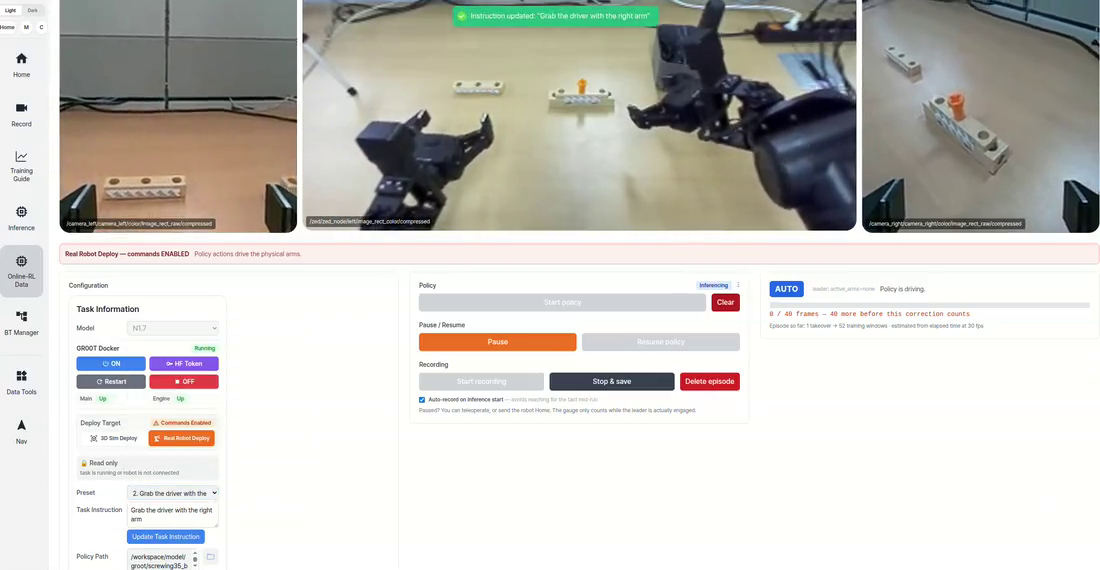
\includegraphics[width=\linewidth]{figs/ui_state_auto.png}
\caption{The policy driving. The banner reads \textsc{auto}, the phase chip reads
inferencing, and \emph{Pause} is the available control. Frames recorded in this
state carry label 0. The toast records a sub-task instruction being changed at a
phase boundary.}
\label{fig:uiauto}
\end{figure}

\begin{figure}[H]
\centering
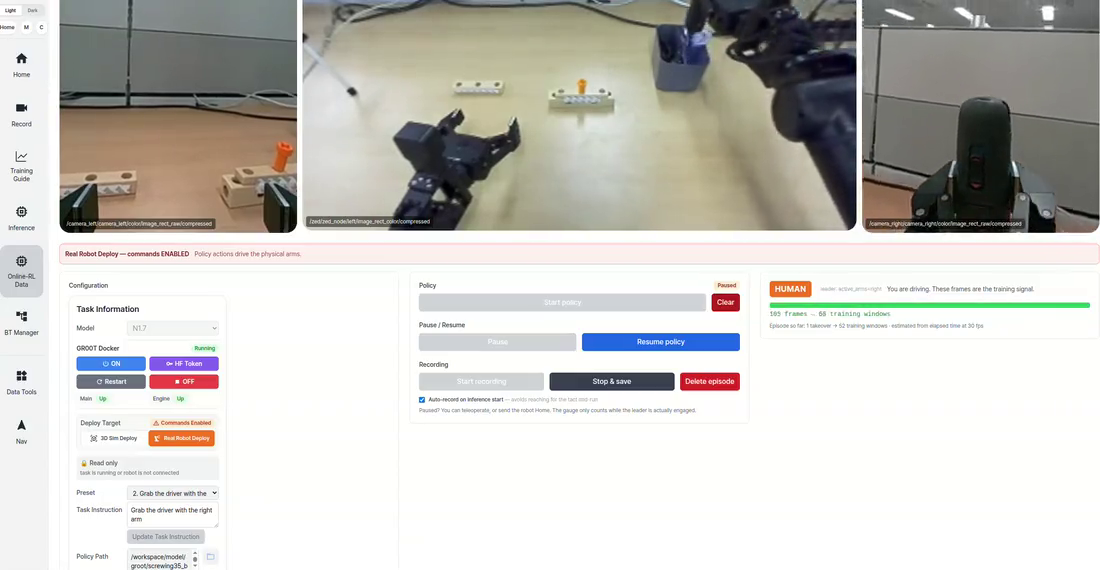
\includegraphics[width=\linewidth]{figs/ui_state_human.png}
\caption{An intervention in progress. The banner reads \textsc{human}, \emph{Resume
policy} is the available control, and the counter reads 105 frames against 66
training windows --- one window for every frame past the fortieth. Frames
recorded in this state carry label 1.}
\label{fig:uihuman}
\end{figure}

The tact switch is a toggle: engagement and release use the same control. The
joystick gesture publishes a single empty message; the orchestrator determines
whether it denotes suspension or resumption from the current phase.

\begin{figure} [H]
    \centering
    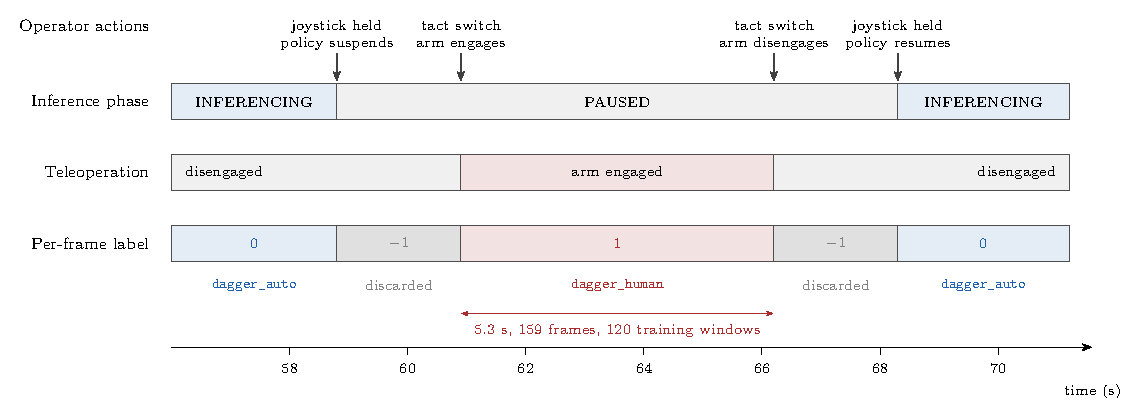
\includegraphics[width=1\linewidth]{figs/intervention_timeline.pdf}
    \caption{One intervention on a time axis:
inference phase, teleoperation engagement, and the resulting per-frame label,
showing the excluded intervals either side of the correction.}
    \label{fig:timeline}
\end{figure}

The intervals between steps 1 and 2, and between steps 3 and 4, have the policy
suspended and no arm engaged. These frames are labelled $-1$ and excluded from
training. No urgency is required at these points.

\remark{In control mode 2, engagement captures a leader anchor and a follower
anchor and thereafter commands
\texttt{goal = follower\_anchor + (leader\_now - leader\_anchor)}.
As the leader is moved, the follower moves in delta from its stopped position. Mode 1 relays absolute leader positions and does exhibit such motion, which is why slow start is enabled in
mode 1 and disabled in mode 2. SG2 uses mode 2 by default.}

\begin{figure}[H]
\centering
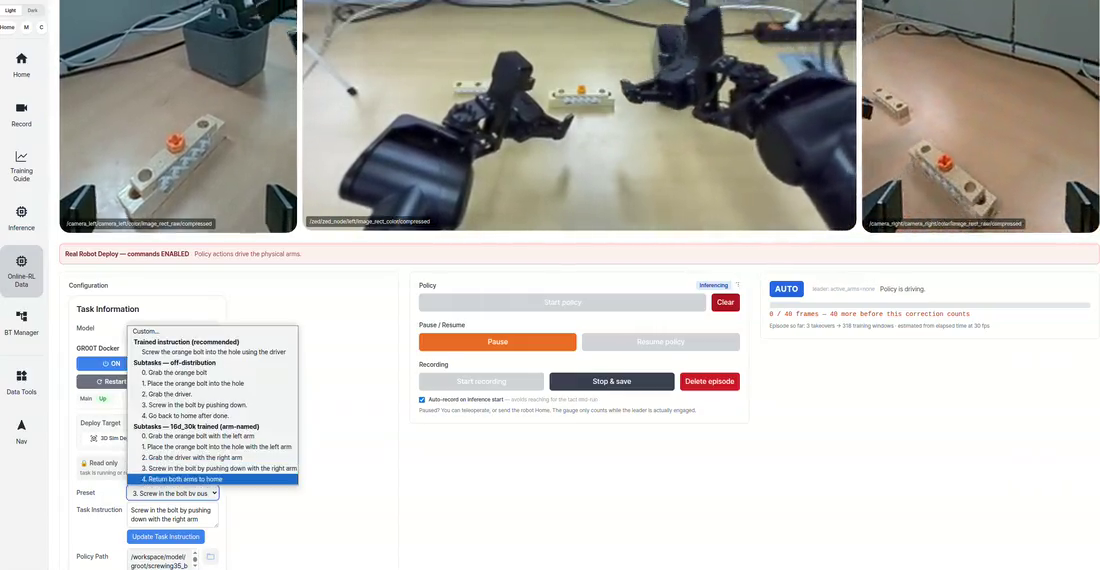
\includegraphics[width=\linewidth]{figs/ui_instruction.png}
\caption{The sub-task instruction control with the list open. The entries correspond
to the phases of the task; the selection made at each phase change is what
divides an episode into correctly timed sub-segments and is written to
\texttt{subtask\_index}.}
\label{fig:uiinstr}
\end{figure}

\subsection{Minimum correction length}

A training sample is a window of forty consecutive frames, corresponding to one
action chunk, rather than an individual frame. A run of $n$ intervened frames
therefore yields at most $n-39$ windows, and a run shorter than forty frames
yields none.

\caution{Sample yield is strongly non-linear in correction length. A run of 45
frames yields 6 windows; a run of 120 frames yields 81. A session composed of
short corrections may convert without error and produce no training data. At
30\,Hz, forty frames is 1.33 seconds; corrections of several seconds are
appropriate. The interface displays a counter against this threshold.}

\subsection{Prohibited actions}

\begin{itemize}
\item The tact switch must not be used to trigger recording while the policy is
      executing. Its recording trigger is disabled on this robot for that
      reason: a single press also engages the corresponding arm, which would
      then publish to the topic the policy is driving.
\item Episodes must not be saved without an outcome. Aggregation admits
      successful episodes only; the operator frames of a failed episode are
      corrections toward an outcome that was not achieved.
\end{itemize}

% =====================================================================
\section{Recorded data}

The robot configuration file is the authoritative specification. Every topic
referenced there is subscribed by the recorder, and the observation topics are
additionally subscribed by the live inference path. This pipeline is comparable to the rosbag2 recorder Cyclo Intelligence offers.

\begin{lstlisting}[style=yml,caption={\texttt{shared/robot\_configs/ffw\_sg2\_rev1\_config.yaml}, abridged}]
observation:
  images:
    cam_left_head:   {topic: /zed/zed_node/left/image_rect_color/compressed}
    cam_left_wrist:  {topic: /camera_left/.../compressed, rotation_deg: 270}
    cam_right_wrist: {topic: /camera_right/.../compressed, rotation_deg: 270}
    cam_right_head:  {topic: /zed/zed_node/right/image_rect_color/compressed}
  state:
    upper_body: {topic: /joint_states}    # 19 joints
    mobile:     {topic: /odom}            # linear_x, linear_y, angular_z

action:
  arm_left:  {topic: /leader/joint_trajectory_command_broadcaster_left/joint_trajectory}
  arm_right: {topic: /leader/joint_trajectory_command_broadcaster_right/joint_trajectory}
  head:      {topic: /leader/joystick_controller_left/joint_trajectory}
  lift:      {topic: /leader/joystick_controller_right/joint_trajectory}
  mobile:    {topic: /cmd_vel}

recording:
  extra_topics:
    - /task/inference_status
    - /tf
    - camera_info topics
\end{lstlisting}
\begin{figure} [H]
    \centering
    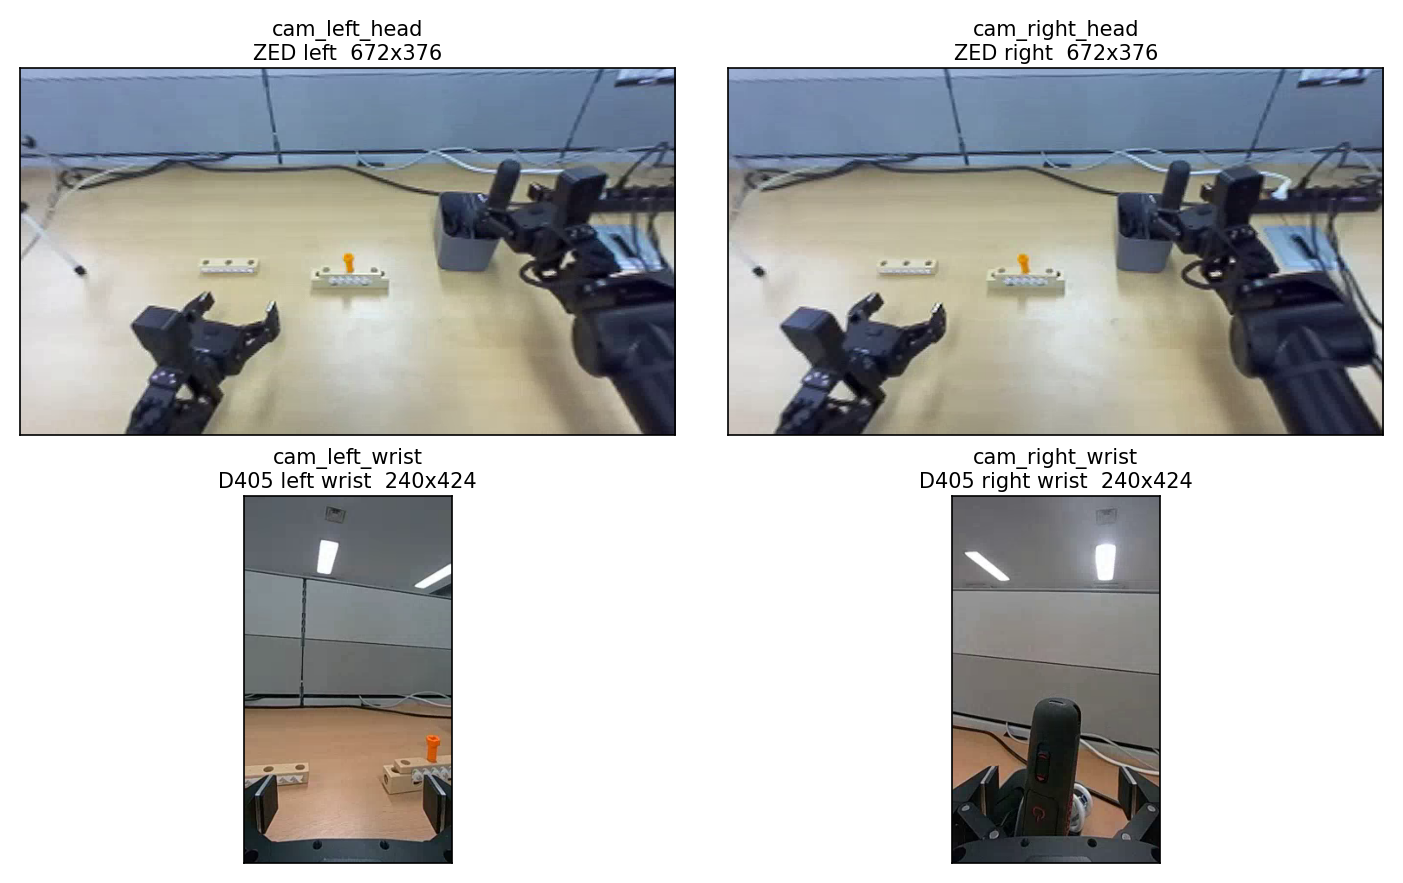
\includegraphics[width=1\linewidth]{figs/camera_views.png}
    \caption{The four recorded camera streams as
captured: head left and right, and the two wrist cameras. Three of the four are
declared to the policy.}
    \label{fig:cameras}
\end{figure}

\subsection{Dimensions}

\begin{center}
\small
\begin{tabular}{@{}lcl@{}}
\toprule
\textbf{Field} & \textbf{Dimensions} & \textbf{Composition}\\
\midrule
\texttt{observation.state} & 22 & 19 upper-body joints, 3 odometry\\
\texttt{action}            & 20 & 16 arm, 1 lift, 3 mobile\\
Declared to the policy     & 16 & Both arms\\
\bottomrule
\end{tabular}
\end{center}

The state vector includes \texttt{head\_joint1} and \texttt{head\_joint2}; the
action vector does not. Slice order follows the insertion order of the
configuration file. The policy is trained on the first sixteen dimensions only;
the remainder are recorded but unused.


\subsection{Image preparation}
\label{sec:crop}

The vision-language backbone stacks the camera views into a single tensor, so
every view presented to it must be square. The four recorded streams are not:
the head camera is 672$\times$376 and the wrist cameras are 240$\times$424. Two
methods reconcile this, and the choice between them is not neutral.

\begin{center}
\small
\begin{tabular}{@{}lp{9.6cm}@{}}
\toprule
\textbf{Method} & \textbf{Effect}\\
\midrule
Letterbox & Pad the shorter axis to square. Field of view is preserved; the padding occupies part of the token budget.\\
Square crop & Crop the longer axis to square. No padding; the cropped region is discarded.\\
\bottomrule
\end{tabular}
\end{center}

\begin{figure}[H]
\centering
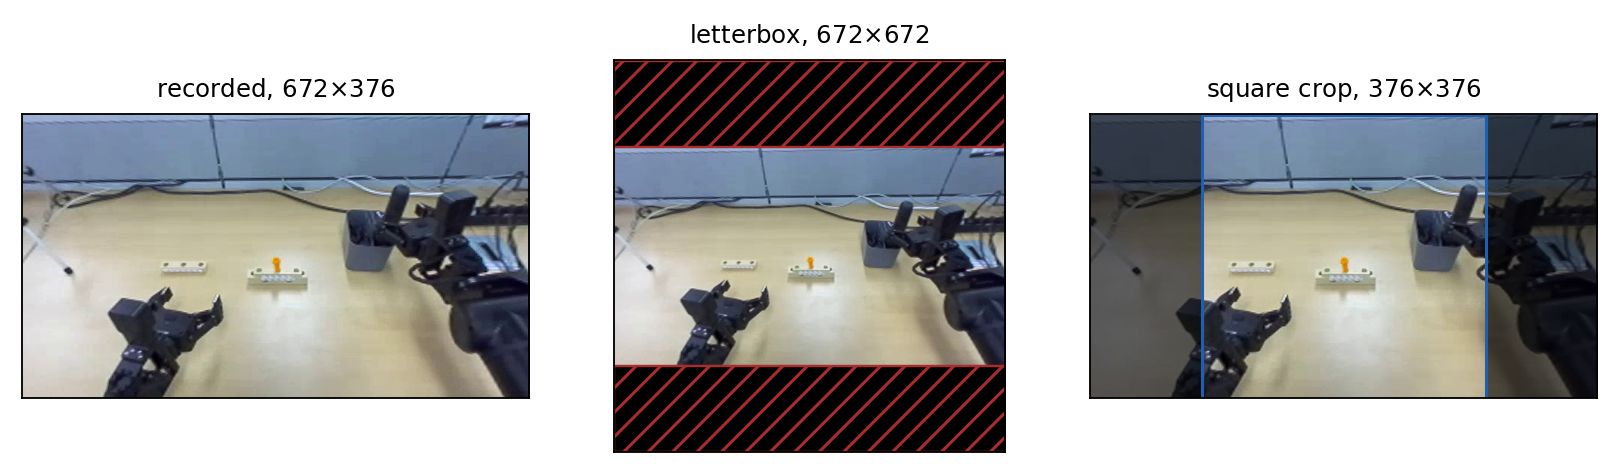
\includegraphics[width=\linewidth]{figs/crop_methods.png}
\caption{The two methods on one head-camera frame. Hatched: padding added.
Darkened: image discarded.}
\label{fig:cropmethods}
\end{figure}

\subsection{Why neither method is applied uniformly}

Letterboxing every view, which is the default behaviour, places 43.6 per cent of
each model input in black bars. Cropping every view to square removes that
waste but discards image. The two camera types were measured separately before
the decision was taken, and they do not behave alike.

\begin{center}
\small
\begin{tabular}{@{}lp{9.4cm}@{}}
\toprule
\textbf{Camera} & \textbf{Measurement}\\
\midrule
Head  & Fixed mounting, so frame-to-frame change is task activity. \textbf{47.8 per cent of its motion energy}, and 67.4 per cent during the driver grasp, lies in the lateral bands a centred square crop would remove.\\
Wrist & Moving mounting, so most frame-to-frame change is background sweeping past the lens; motion energy does not measure task content here. By spatial detail, the band a bottom-anchored crop removes is \textbf{43.4 per cent of the frame carrying 38.7 per cent of its gradient energy}, which is close to proportionate. These are also the cameras with the finest resolution on the workspace, at 0.73 to 1.08\,mm per pixel.\\
\bottomrule
\end{tabular}
\end{center}

\begin{figure}[H]
\centering
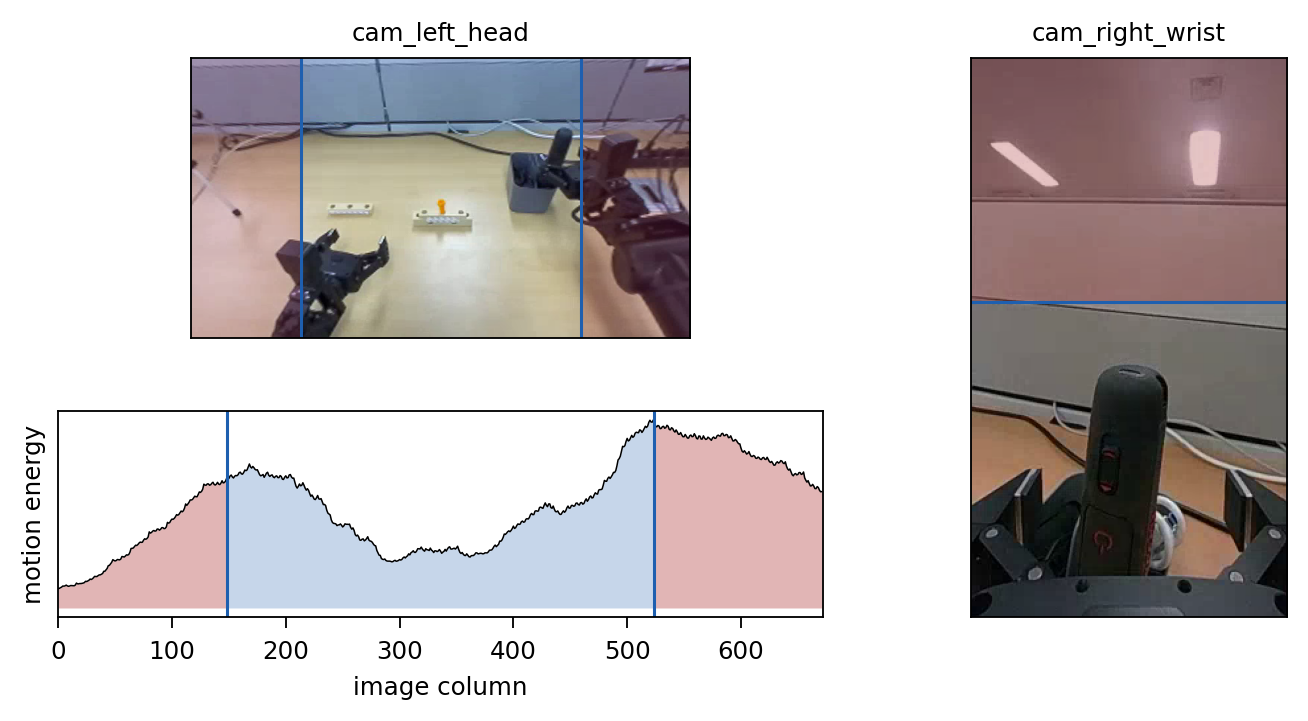
\includegraphics[width=0.8\linewidth]{figs/crop_evidence.png}
\caption{Shaded regions are what a square crop would remove. Left, the head
camera and its column-wise motion energy; right, the wrist camera and its
bottom-anchored crop line.}
\label{fig:cropevidence}
\end{figure}

A centred square crop of the head camera would therefore remove the columns in
which the work occurs. The wrist cameras carry no equivalent argument in either
direction; the case for cropping them is the padding it avoids and the held-out
measurement in Section~\ref{sec:cropeval}.

\remark{These quantities were measured over episode~0 of the reference session,
3{,}423 frames, sampled every fourth frame. They are measurements of one
episode in one scene and should be regenerated if the cell is rearranged. The
regeneration script is \texttt{scripts/crop\_stats.py}.}

\subsection{The applied configuration}

Each view must be square, but the squares need not be of equal size: a trailing
resize normalises all of them to 256$\times$256 before they are stacked.

\begin{center}
\small
\begin{tabular}{@{}llll@{}}
\toprule
\textbf{Camera} & \textbf{Source} & \textbf{Prepared} & \textbf{Padding}\\
\midrule
\texttt{cam\_left\_head}   & 672$\times$376, full frame     & 672$\times$672 & 44.0\,\%\\
\texttt{cam\_left\_wrist}  & 240$\times$240, rows 184--424  & 240$\times$240 & 0\,\%\\
\texttt{cam\_right\_wrist} & 240$\times$240, rows 184--424  & 240$\times$240 & 0\,\%\\
\bottomrule
\end{tabular}
\end{center}

The head is letterboxed and retains its full field of view; the wrist crops are
anchored to the lower edge, which removes the ceiling. Across all views:

\begin{center}
\small
\begin{tabular}{@{}lrr@{}}
\toprule
& \textbf{Uniform letterbox} & \textbf{Applied configuration}\\
\midrule
Head padding              & 44.0\,\% & 44.0\,\%\\
Wrist padding, each       & 43.4\,\% & 0\,\%\\
Mean over the three views & 43.6\,\% & 14.7\,\%\\
\bottomrule
\end{tabular}
\end{center}

The saving comes entirely from the wrist cameras; the head view is unchanged.
These are geometric quantities and follow from the source resolutions alone.

\begin{figure}[H]
\centering
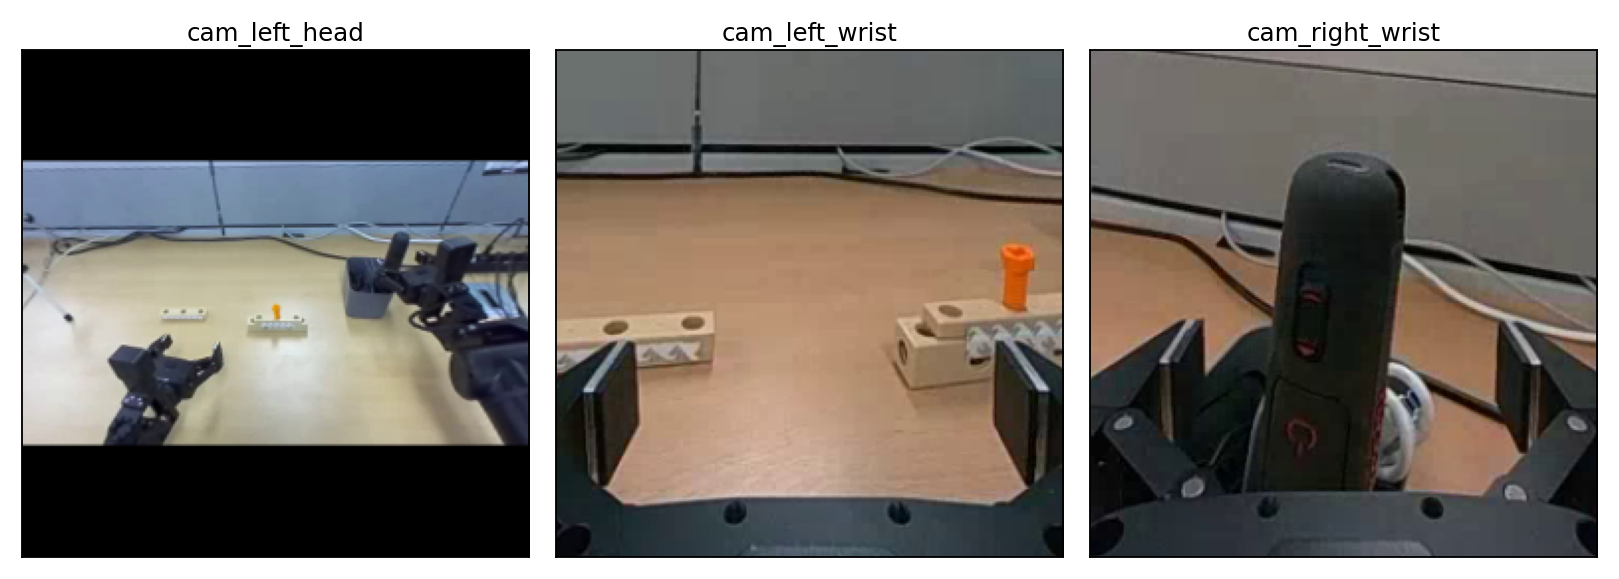
\includegraphics[width=\linewidth]{figs/crop_applied.png}
\caption{The three views as the model receives them, after preparation and the
trailing resize to 256$\times$256.}
\label{fig:cropapplied}
\end{figure}

\subsection{Effect on held-out accuracy}
\label{sec:cropeval}

Measured under an identical protocol, on the same held-out episodes, by forward
kinematics over the final sixty frames of each phase.

\begin{center}
\small
\begin{tabular}{@{}lrr@{}}
\toprule
& \textbf{Uniform letterbox} & \textbf{Applied configuration}\\
\midrule
Grasp the bolt, left arm    & 16.3\,mm & 14.4\,mm\\
Grasp the driver, right arm & 22.7\,mm & 13.3\,mm\\
Systematic fraction, right  & 0.87     & 0.40\\
\bottomrule
\end{tabular}
\end{center}

The systematic fraction is the ratio of the mean bias to the mean error. A value
near unity indicates a fixed offset, which no amount of averaging removes; 0.40
indicates that most of the residual is noise. This configuration was in effect
for the checkpoint that first grasped reliably on hardware.

\caution{The configuration is specified in \texttt{configs/roi\_hybrid.json} and
applied by \texttt{crop\_to\_square.patch}, which is not present in a fresh
clone of Isaac-GR00T. Without the patch every camera is letterboxed and the
inputs no longer match those the checkpoint was trained on. The training
launcher verifies the patch before starting.}

\subsection{Attention over the prepared views}

The action expert cross-attends to the image tokens at eight of the diffusion
transformer's blocks, over four denoising steps. Each view is 8$\times$8 tokens,
192 in all; the values are averaged over heads and over the action queries and
aggregated across those 32 captures. Each panel is normalised over its own 64
tokens, so colour is comparable within a panel and not between panels.

The same checkpoint was run twice on one frame of the place-in-hole phase,
once under the applied crop and once with every view letterboxed. Only the image
preparation differs between the two: the frame, the state and the language
instruction are identical, and the figure asserts that before it is drawn.

\begin{center}
\small
\begin{tabular}{@{}lrr@{}}
\toprule
& \textbf{Applied crop} & \textbf{Uniform letterbox}\\
\midrule
Normalised entropy over the 192 tokens & 0.9851 & 0.9885\\
Share held by the 8 strongest tokens   & 9.1\,\% & 8.4\,\%\\
Padding's share of the token grid      & 16.7\,\% & 50.0\,\%\\
Attention landing on padding           & 18.9\,\% & 48.8\,\%\\
\bottomrule
\end{tabular}
\end{center}

A uniform distribution would give the eight strongest tokens 4.2 per cent, and
would put exactly as much attention on padding as padding holds of the grid.
Both configurations sit close to that: the last two rows differ by around two
percentage points each. Letterboxing does not make the policy attend to black
bars in preference to the workspace; it gives it three times as many of them to
spread over, and the wrist views lose the workpiece to ceiling and wall in the
process.

\remark{All five phases of the episode were measured, not only the one shown.
The additional attention spent on padding under a uniform letterbox ranges from
25.8 per cent at the bolt grasp to 30.8 per cent at the home pose, against 29.8
per cent here. The effect is a property of the token grid rather than of the
frame, so the figure is representative of the episode and not the best case in
it.}

\caution{The checkpoint was trained under the applied crop, so the letterbox
rows are the model running on inputs it was never fitted to. They show what the
preparation costs, not what a policy trained on letterboxed views would do.
Attention this flat does not identify what the policy uses either way, and was
not used to choose the crop; the grounds are the motion-energy measurements of
Section~\ref{sec:crop} and the held-out error of Section~\ref{sec:cropeval}.}

\begin{figure}[H]
\centering
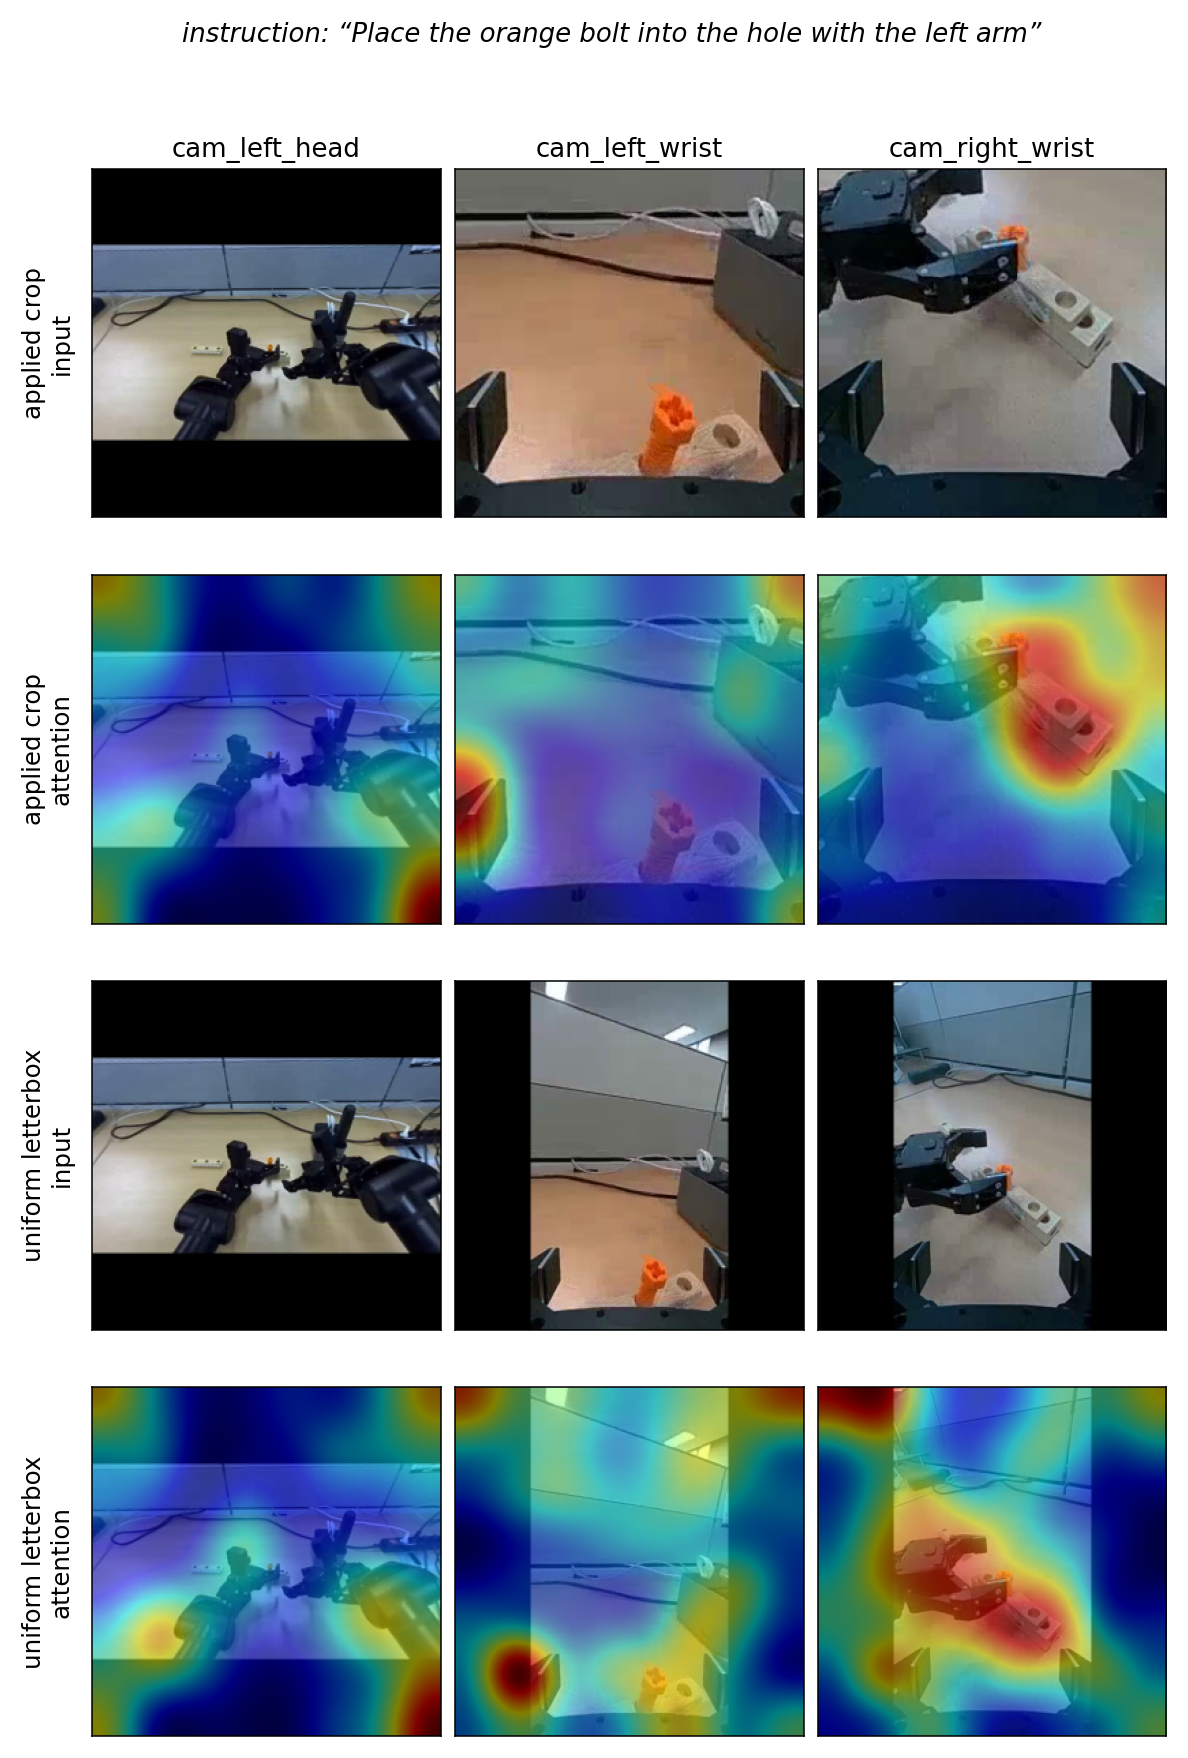
\includegraphics[width=0.72\linewidth]{figs/attn_map.png}
\caption{Image cross-attention as the bolt is placed into the hole,
checkpoint 30{,}000, under the two image preparations. Rows one and two are the
applied crop, rows three and four the uniform letterbox; within each pair the
first row is the views as the model receives them and the second the same views
with the attention overlaid. The language instruction, shown above, was the same
in both runs. Each panel is min-max normalised over its own 64 tokens, so red
marks that panel's strongest tokens and is not comparable between panels.}
\label{fig:attnmap}
\end{figure}

% =====================================================================
\newpage
\section{The intervention label}
\label{sec:defect}

\subsection{Derivation}

\texttt{/task/inference\_status} publishes the inference phase on transitions
only. The converter forward-fills it onto the frame grid and assigns:

\begin{center}
\small
\begin{tabular}{@{}ll@{}}
\toprule
\textbf{Condition} & \textbf{Label}\\
\midrule
Inferencing                                  & 0\\
Paused, teleoperation engaged, not a handoff & 1\\
Paused, teleoperation not engaged            & $-1$\\
Handoff transient                            & $-1$\\
Prior to the first status message            & $-1$\\
\bottomrule
\end{tabular}
\end{center}

Label 0 denotes the policy, label 1 the operator, and $-1$ exclusion.

\subsection{Emitted columns}

Conversion has two writers, selected by the format flags on T13:
\texttt{to\_lerobot\_v21.py} produces LeRobot v2.1, which is the layout
Isaac-GR00T requires, and \texttt{to\_lerobot\_v30.py} produces v3.0. Both emit
the label, together with three further columns belonging to the online-RL
schema. The values are attached to the episode structure during conversion, so
neither writer performs any additional computation.

Neither set of columns belongs to stock LeRobot. The format permits additional
columns, and this converter already relies on that: \texttt{subtask\_index},
which divides an episode into sub-segments, is likewise not part of the
published specification.

\begin{center}
\small
\begin{tabular}{@{}lll@{}}
\toprule
\textbf{Column} & \textbf{Type} & \textbf{Contents}\\
\midrule
\texttt{intervention}   & int64   & 1 operator, 0 policy, $-1$ excluded\\
\texttt{reward}         & int64   & Per-frame return\\
\texttt{done}           & bool    & Terminal frame of an episode\\
\texttt{sample\_weight} & float32 & Per-frame training weight\\
\bottomrule
\end{tabular}
\end{center}

\begin{lstlisting}[style=py,caption={Schema block, common to both writers}]
has_hil_feature = any(ep.intervention_flags for ep in episodes)
if has_hil_feature:
    schema_fields.append(pa.field("intervention",  pa.int64()))
    schema_fields.append(pa.field("reward",        pa.int64()))
    schema_fields.append(pa.field("done",          pa.bool_()))
    schema_fields.append(pa.field("sample_weight", pa.float32()))
\end{lstlisting}

The columns are written only where \texttt{/task/inference\_status} was present
in the recording. An ordinary teleoperation session produces none of them, and
their absence is not by itself a fault.

Each column is declared in \texttt{meta/info.json} as well as written to the
parquet files. The declaration is not optional: tooling that reads the feature
list will not observe a column present only in the parquet.

\remark{Of the four, only \texttt{intervention} governs the procedure in this
manual. \texttt{reward} and \texttt{done} belong to reinforcement learning
rather than HG-DAgger, and \texttt{sample\_weight} cannot be acted upon by
Isaac-GR00T, which provides no per-frame loss weighting; that weighting is
applied at the dataset level instead, as described in
Section~\ref{sec:mixture}. The four are emitted together because they derive
from one source.}
% =====================================================================
% =====================================================================
\section{HG-DAgger training}
\label{sec:train}

What follows is the continuation run only. It consumes the session recorded in
Section~\ref{sec:loop}, the original demonstrations the base policy was fitted
to, and the base checkpoint of Section~\ref{sec:base}.

\subsection{Procedure}

The sequence below takes a converted session through to a selected checkpoint.
Paths are written relative to the training root.

\begin{lstlisting}[style=sh]
# 1. Validate the converted dataset. Refuses on a degenerate normaliser.
python3 scripts/verify_dataset.py --root datasets/<session> --isaac

# 2. If the export lacks the intervention column, repair it first.
#    Idempotent; backs up whatever it replaces.
python3 scripts/fix_dagger_dataset.py \
    --root datasets/<session> \
    --reference datasets/screwing35_follower_val

# 3. Inspect the partition before writing it.
python3 configs/export_dagger_split.py \
    --src datasets/<session> --out-dir datasets/ --dry-run

# 4. Write the partition. Each intervention becomes its own episode and the
#    video is cut by frame index.
python3 configs/export_dagger_split.py \
    --src datasets/<session> --out-dir datasets/

# 5. Validate both outputs. Video was re-encoded, so the alignment check
#    is the one that matters here.
python3 scripts/verify_dataset.py --root datasets/dagger_human --isaac
python3 scripts/verify_dataset.py --root datasets/dagger_auto  --isaac

# 6. Train.
ROOT=$PWD \
BASE=$PWD/runs/16d_30k/checkpoint-30000 \
ORIG=$PWD/datasets/screwing35_follower_train \
HUMAN=$PWD/datasets/dagger_human \
AUTO=$PWD/datasets/dagger_auto \
GR=$PWD/Isaac-GR00T \
NUM_GPUS=2 STEPS=6000 \
bash configs/06_train_dagger.sh

# 7. Select a checkpoint by held-out error, not by training loss.
python3 scripts/checkpoint_sweep.py \
    --runs runs/groot_dagger_it1 \
    --dataset datasets/screwing35_follower_val \
    --v30     datasets/screwing35_follower_val
\end{lstlisting}

\caution{Step 6 prints a mixture line at start-up. It must list three
specifications at the intended ratios. A single specification indicates that
\texttt{mixture\_ratio.patch} was not applied and that the datasets are being
weighted by size.}

\subsection{Dataset partition}
\label{sec:mixture}

Isaac-GR00T provides no per-frame loss weighting. The frame-level weighting
scheme is therefore approximated at the dataset level using mixture ratios, and
the partition is performed at export time. For instance:

\begin{center}
\small
\begin{tabular}{@{}lrrr@{}}
\toprule
\textbf{Dataset} & \textbf{Episodes} & \textbf{Frames} & \textbf{Ratio}\\
\midrule
Original demonstrations & 31 & 55{,}701 & 0.60\\
Operator corrections    & 39 & 6{,}765  & 0.30\\
Policy frames           & 52 & 31{,}804 & 0.10\\
\bottomrule
\end{tabular}
\end{center}

Each intervention is exported as an independent episode. Video is indexed per
episode and the policy consumes action chunks; concatenating two interventions
into one episode would introduce a transition that did not occur.

\caution{In the absence of explicit ratios the loader weights datasets by size.
The corrections are 6{,}765 frames of the 94{,}270 in the mixture and would
therefore receive 7 per cent of it rather than 30. The mixture line in the
launch log should be checked against the intended ratios.}

\begin{figure}[H]
\centering
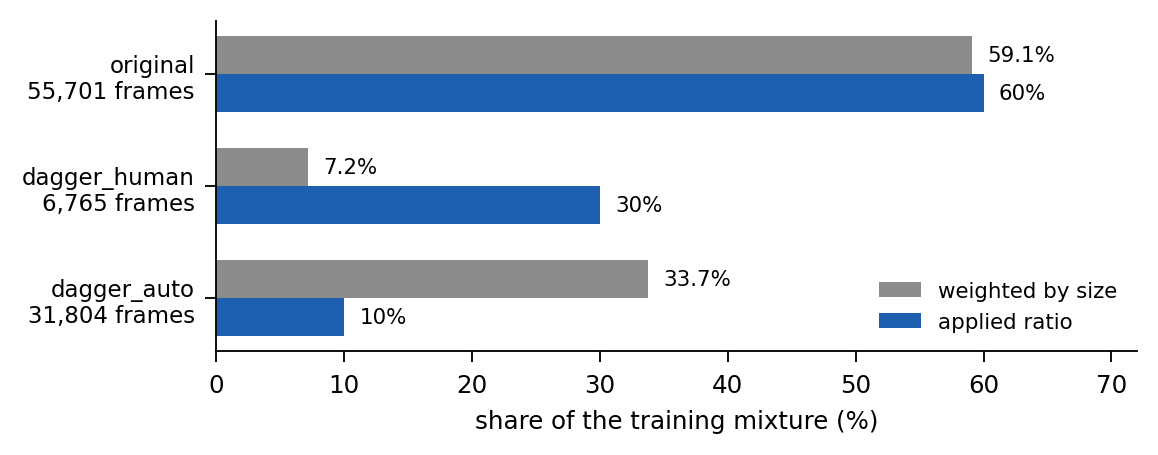
\includegraphics[width=0.85\linewidth]{figs/mixture_proportions.png}
\caption{Each dataset's share of the training mixture: what weighting by size would
give, against the ratios actually applied. The corrections are the only ones
that move materially, from 7 per cent to 30.}
\label{fig:mixture}
\end{figure}

\subsection{Warm start}

The base checkpoint contains weights only. No optimiser state is present and its
cosine schedule has annealed to approximately $3 \times 10^{-13}$, so there is
nothing to resume; the continuation is a fresh schedule over pretrained weights.
The learning rate is the one parameter that must change. At the base run's
$1 \times 10^{-4}$ a converged checkpoint is driven out of its basin within the
first few hundred steps.

\begin{center}
\small
\begin{tabular}{@{}lll@{}}
\toprule
\textbf{Parameter} & \textbf{Base run} & \textbf{Continuation}\\
\midrule
Learning rate  & $1 \times 10^{-4}$ & $3 \times 10^{-5}$\\
Global batch   & 128 & 128\\
Frozen         & Language and vision & Language and vision\\
Trained        & Projector, diffusion head & Projector, diffusion head\\
State dropout  & 0.2 & 0.2\\
\bottomrule
\end{tabular}
\end{center}

\subsection{Step budget}

The step count should be selected by dataset exposure rather than elapsed time.

\begin{center}
\small
\begin{tabular}{@{}rrrr@{}}
\toprule
\textbf{Steps} & \textbf{Original} & \textbf{Corrections} & \textbf{Duration}\\
\midrule
1{,}500  & 2.1$\times$  & 8.5$\times$ & 0.4\,h\\
3{,}000  & 4.1$\times$  & 17$\times$  & 0.8\,h\\
6{,}000  & 8.3$\times$  & 34$\times$  & 1.5\,h\\
\bottomrule
\end{tabular}
\end{center}

Exposure is counted as steps $\times$ batch $\times$ the dataset's mixture
ratio, divided by its frame count. The architecture tolerates a good deal of
repetition, since diffusion training injects noise at every step and state
dropout regularises further; the base run reached 68.9 epochs over the original
data without degrading. The correction set does not have that latitude.
Thirty-nine runs from a single scene, repeated several hundred times, are
memorised rather than learned, which is what bounds the budget above.

\begin{figure}
    \centering
    \includegraphics[width=0.8\linewidth]{trainingloss.png}
    \caption{Training loss for HG-DAgger Iteration ($n=1$)}
    \label{fig:trainloss}
\end{figure}

\subsection{Checkpoint selection}

Evaluation must be performed in Cartesian space. A seven-degree-of-freedom arm
attains a given position through many joint configurations, so joint-space error
is a poor proxy for end-effector accuracy. Select by held-out error rather than
by training loss: a small correction set is readily memorised, and training loss
continues to fall after held-out performance has turned.

The series below is the base run's own sweep, shown because it is the one that
survives; the procedure is identical for the continuation's checkpoints.

\begin{figure}[H]
\centering
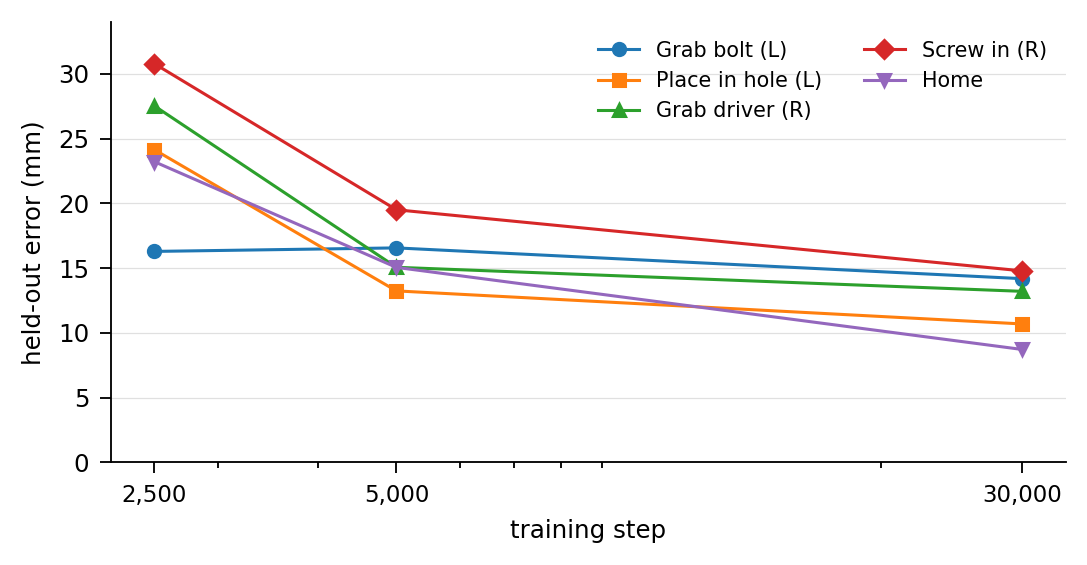
\includegraphics[width=0.78\linewidth]{figs/checkpoint_sweep.png}
\caption{Held-out Cartesian error against training step, one series per task phase,
measured by forward kinematics over the last sixty frames of each phase on the
four held-out episodes.}
\label{fig:sweep}
\end{figure}

% =====================================================================
\section{Deployment}
\label{sec:deploy}

\subsection{Transferring the checkpoint}

Checkpoints are published to Hugging Face rather than copied between machines.

\begin{center}
\small
\begin{tabular}{@{}ll@{}}
\toprule
\textbf{Repository} & \textbf{Contents}\\
\midrule
\texttt{dawity/groot\_screwing35}  & Base checkpoints, including the 16-dimension 30k model\\
\texttt{dawity/groot\_dagger\_it1} & Checkpoints from the first HG-DAgger continuation\\
\bottomrule
\end{tabular}
\end{center}

\begin{lstlisting}[style=sh]
huggingface-cli download dawity/groot_dagger_it1 \
    --include "checkpoint-6000/*" --local-dir /workspace/model/groot/
\end{lstlisting}

A checkpoint comprises fifteen files. A directory containing fewer than fifteen
is an incomplete transfer and will fail to load; the file count should be
confirmed before deployment.

\subsection{Configuration that must match training}

\caution{The following are properties of the checkpoint, not of the deployment,
and a mismatch produces degraded behaviour rather than an error.}

\begin{center}
\small
\begin{tabular}{@{}lll@{}}
\toprule
\textbf{Property} & \textbf{Value} & \textbf{Consequence of mismatch}\\
\midrule
Declared dimensions & 16, both arms      & Input is scaled incorrectly\\
Cameras             & 3 of the 4 recorded & An unseen view is supplied\\
Crop                & Per-camera, \texttt{roi\_hybrid.json} & Framing differs from training\\
\texttt{crop\_fraction} & 1.0            & Random cropping is reintroduced\\
\texttt{use\_percentiles} & false        & Normalisation differs\\
Action horizon      & 40                 & Chunk length differs\\
\bottomrule
\end{tabular}
\end{center}

The last two are read from the checkpoint's own configuration and are already
correct in the published checkpoints. The camera selection and crop are
deployment-side settings and must be set to match.

\subsection{Bringing the policy up}

\begin{enumerate}
\item Start the follower, the leader and the bridge as in Section~\ref{sec:bringup}.
\item Set the policy path in the operator interface to the downloaded
      checkpoint directory.
\item Load the policy. The phase indicator moves from ready through loading to
      inferencing.
\item Confirm that commands are enabled before expecting motion. The interface
      distinguishes a loaded policy from one that is driving the arms.
\end{enumerate}

\begin{figure}[H]
\centering
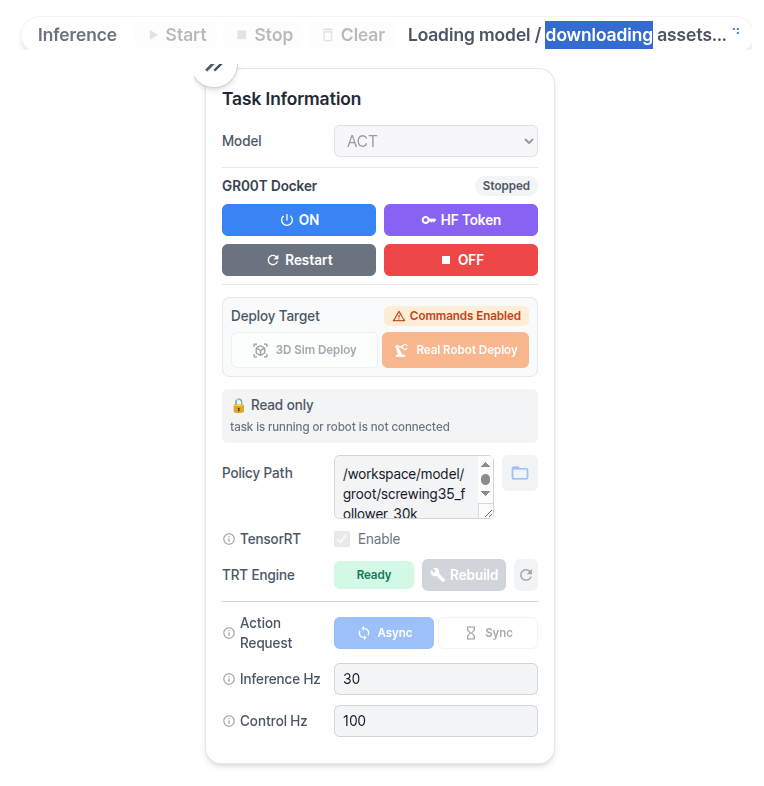
\includegraphics[width=0.52\linewidth]{figs/ui_policy_load.png}
\caption{The policy loading. The header reads \emph{Loading model / downloading
assets}, the policy path is set to the downloaded checkpoint directory, and the
TensorRT engine reports ready. The arms are not yet being driven.}
\label{fig:uiload}
\end{figure}

\subsection{Control parameters}

The deployed controller applies smoothing and rate limiting on top of the
policy's output.

\begin{center}
\small
\begin{tabular}{@{}lll@{}}
\toprule
\textbf{Parameter} & \textbf{Value} & \textbf{Function}\\
\midrule
Chunk length        & 50 & Actions produced per inference\\
Executed            & 25 & Actions executed before replanning\\
Blend               & 20 & Cubic overlap between successive chunks\\
Smoothing window    & 9  & Savitzky--Golay window\\
Velocity clamp      & 0.6\,rad/s & Limit against the previous command\\
Acceleration clamp  & 2.0\,rad/s\textsuperscript{2} & Limit on commanded acceleration\\
\bottomrule
\end{tabular}
\end{center}

\begin{figure}[H]
\centering
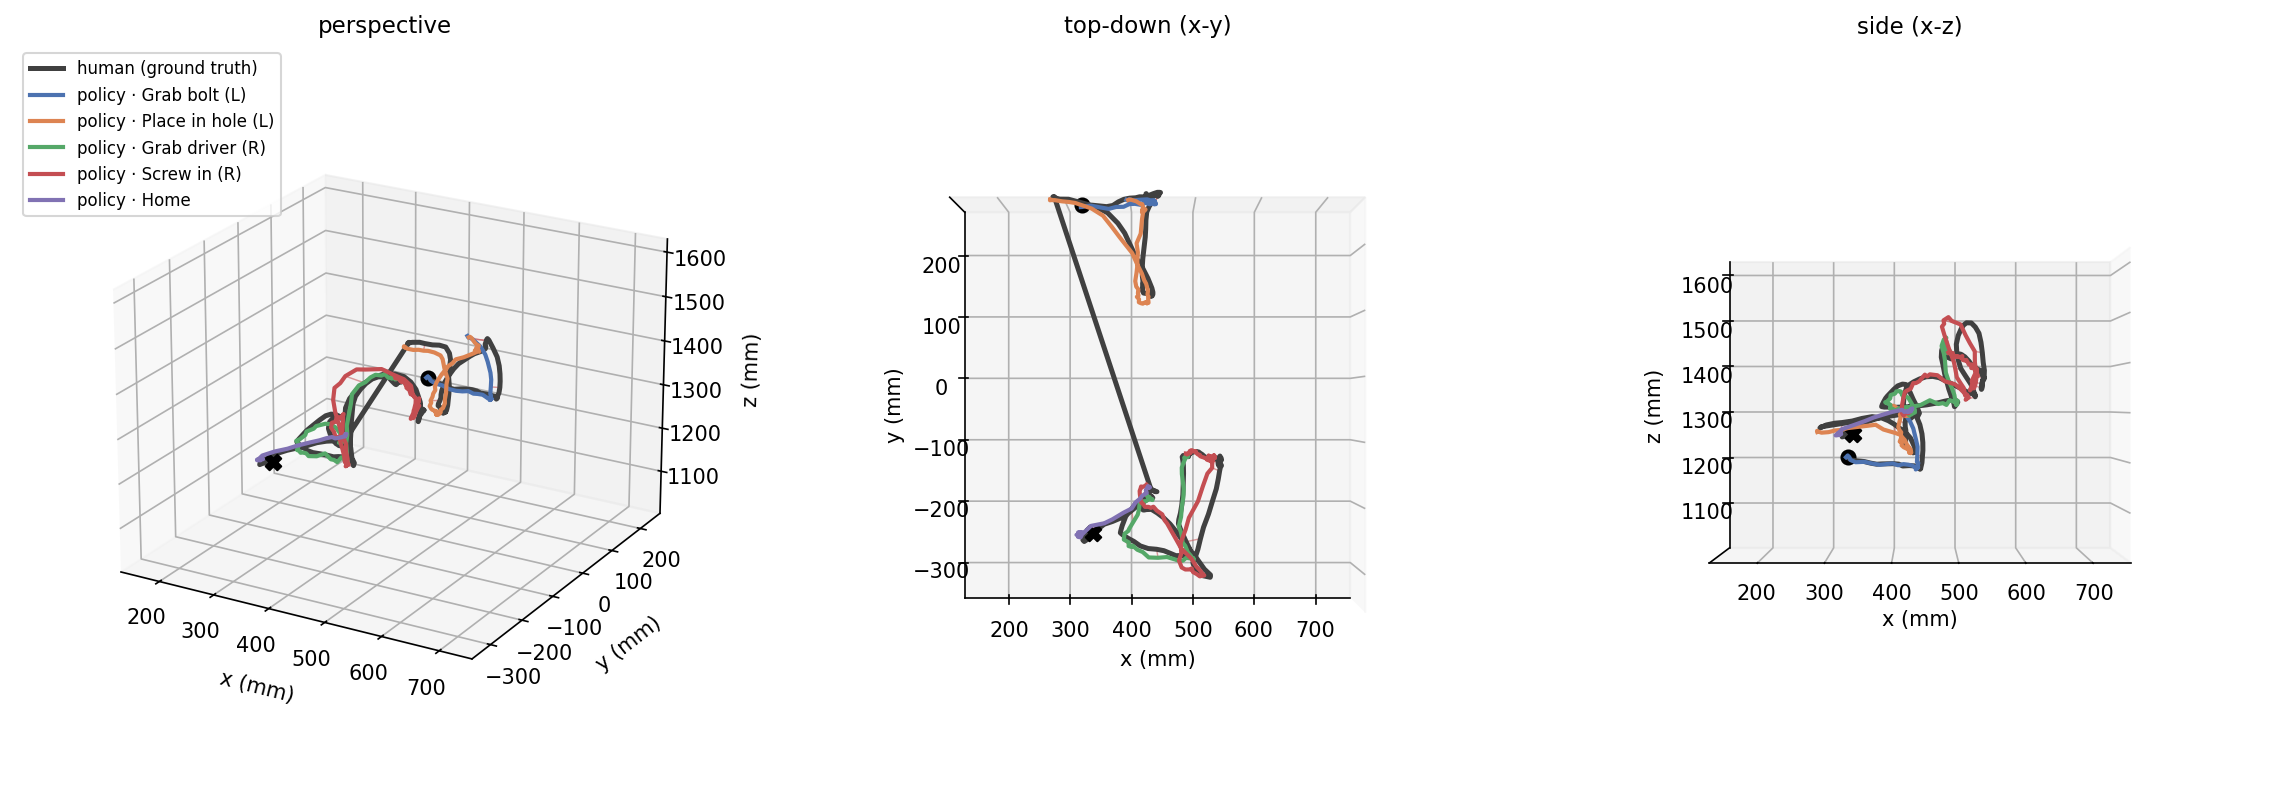
\includegraphics[width=\linewidth]{figs/rollout3d.png}
\caption{Open-loop Cartesian rollout over one held-out episode, in three views. The
dark line is the demonstrated end-effector path and the coloured segments are
the policy's, one colour per task phase; the thin red segments join each
commanded point to the demonstrated one at the same instant.}
\label{fig:rollout}
\end{figure}

\subsection{Evaluation on hardware}

\caution{Offline metrics do not establish robot behaviour. Held-out evaluation
measures agreement with the original demonstrations, and a correction is by
definition a departure from them, so a policy that has learned the corrections
may score worse. Hardware execution is the only measurement that distinguishes
the two cases.}

Where a task fails on hardware, the first measurement to take is whether the arm
reaches the position the policy commanded. A trace of commanded against achieved
position separates a policy error from a control or mechanical one. Additional
training data cannot correct the latter.

\begin{figure}[H]
\centering
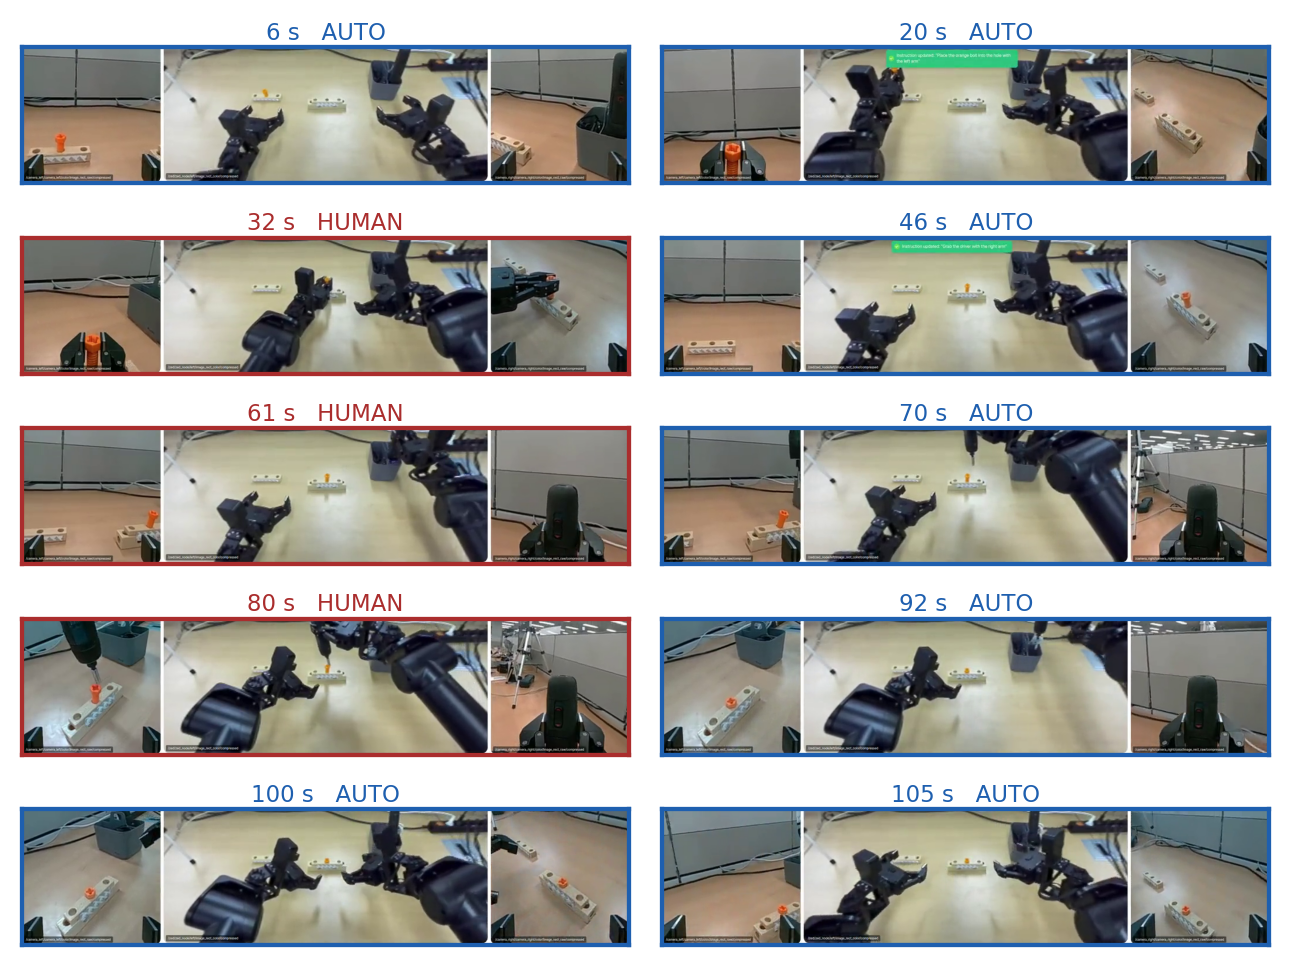
\includegraphics[width=\linewidth]{figs/hardware_rollout.png}
\caption{The session on the physical robot, sampled across its 116 seconds. Each
panel shows the three camera views at that instant, bordered and labelled by
which side was driving. The three red panels fall inside the operator's
takeovers, at 31--34, 58.5--64.5 and 78--84 seconds.}
\label{fig:hwrollout}
\end{figure}

% =====================================================================
\newpage
\section{Verification}
\label{sec:verify}

\subsection{Dataset validation}

\begin{lstlisting}[style=sh]
python3 scripts/verify_dataset.py --root <dataset> --isaac
\end{lstlisting}

\begin{center}
\small
\begin{tabular}{@{}ll@{}}
\toprule
\textbf{Check} & \textbf{Detects}\\
\midrule
Action frame offset   & Action misaligned from the state it follows\\
Freeze frames         & Stationary arm under a label commanding motion\\
Label consistency     & Inconsistent phase semantics across episodes\\
Camera shapes         & Unannounced resolution change\\
Modality declaration  & Dimensions declared but not supplied\\
Normaliser            & Declared dimension of zero range\\
Dataset version       & Layout not matching the required version\\
Video alignment       & Video and parquet disagreeing after re-encoding\\
\bottomrule
\end{tabular}
\end{center}

\begin{figure}[H]
\centering
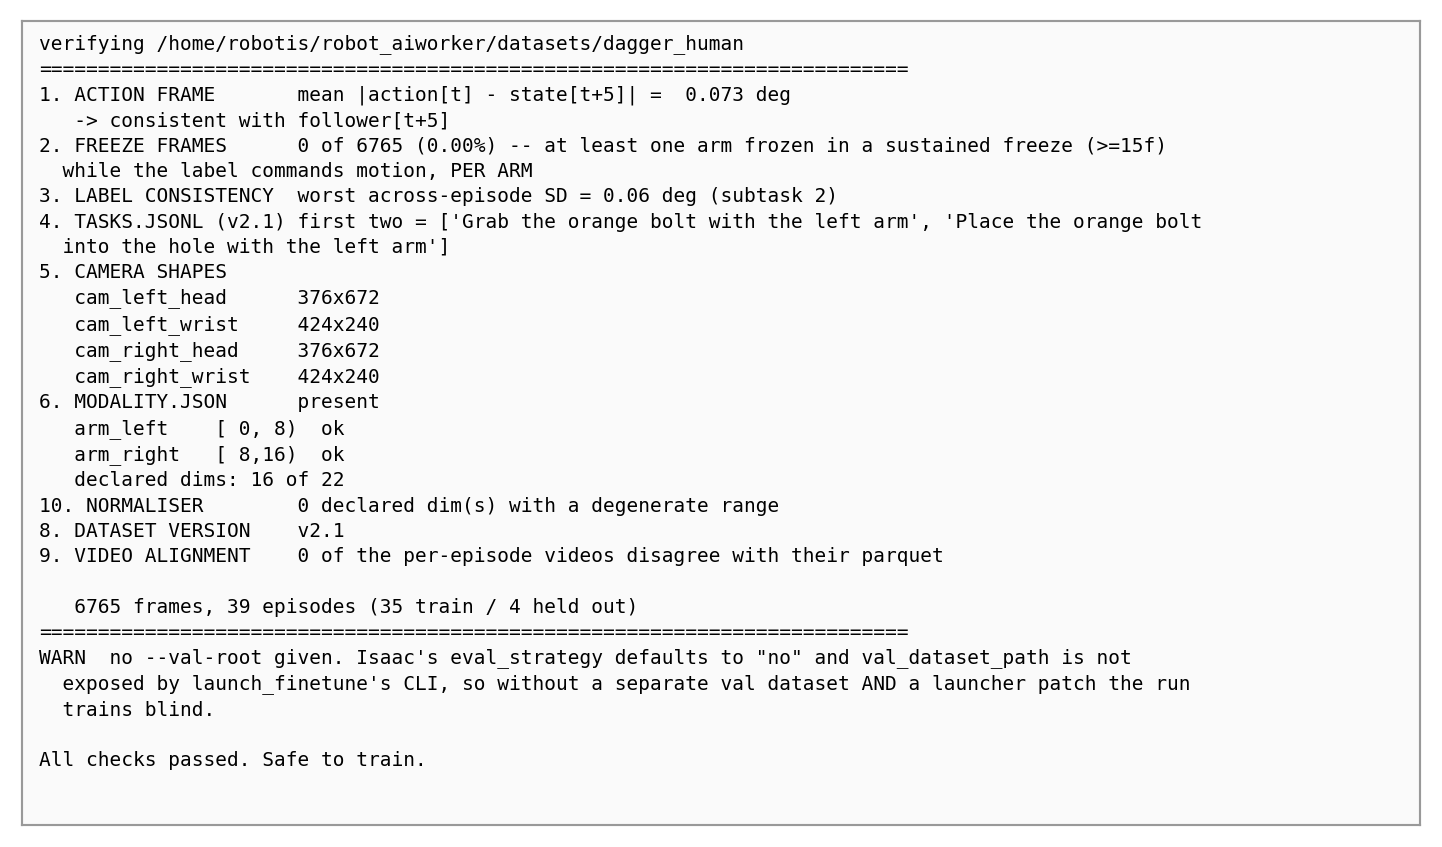
\includegraphics[width=\linewidth]{figs/verify_output.png}
\caption{A passing \texttt{verify\_dataset} report over \texttt{dagger\_human}. The
normaliser and video-alignment checks are the two that most often fail. The
closing warning concerns the absence of a separate validation set, not a fault
in the dataset.}
\label{fig:verify}
\end{figure}

\subsection{Post-conversion assertion}

\begin{lstlisting}[style=py]
import pandas as pd, glob, json
df = pd.concat([pd.read_parquet(f)
                for f in glob.glob("<ds>/data/**/*.parquet", recursive=True)])
assert "intervention" in df.columns
assert "intervention" in json.load(open("<ds>/meta/info.json"))["features"]
print(df.intervention.value_counts())
\end{lstlisting}

All three label values should be present. On the reference session they were
6{,}765 operator frames, 32{,}192 policy frames and 4{,}729 excluded, of 43{,}686.

\caution{Two conventions exist and they are inverses.
\texttt{intervention} uses 1 for the operator and 0 for the policy;
\texttt{task\_is\_policy}, written by older exports, uses 1 for the policy and 0
for the operator. Both use $-1$ for exclusion. A dataset carrying the second
fails the assertion above rather than passing on the complement of the intended
frames, which is why the assertion names the field.}

% =====================================================================
\section{Topic and service reference}
\label{sec:legend}

Numbered notes are given in Section~\ref{sec:legendnotes}.

{\small
\begin{longtable}{@{}llllc@{}}
\toprule
\textbf{ID} & \textbf{Kind} & \textbf{Name} & \textbf{Function} & \textbf{Note}\\
\midrule
\endhead
T1  & Topic          & \texttt{tact\_trigger}          & Tact switch event            & 1\\
T2  & Topic          & \texttt{joystick\_command}      & Arm engage toggle            & 2\\
T3  & Topic          & \texttt{raw\_joint\_trajectory} & Leader arm command           & \\
T4  & Topic          & \texttt{control\_status}        & Active arms and mode         & 3\\
T5  & Topic, latched & \texttt{active\_arms\_str}      & Active arms, string form     & 3\\
T6  & Topic          & \texttt{joint\_trajectory}      & Arm command to the follower  & 4\\
T7  & Topic          & \texttt{joint\_states}, cameras & Observation                  & 5\\
T8  & Topic          & \texttt{engine\_command}        & Policy load and run          & \\
T9  & Service        & \texttt{/task/command}          & Policy and recording control & \\
T10 & Topic, latched & \texttt{inference\_status}      & Inference phase              & 6\\
T11 & Service        & \texttt{/data/recording}        & Recording lifecycle          & \\
T13 & Service        & \texttt{/data/convert}          & Dataset conversion           & 7\\
T14 & Topic, latched & \texttt{policy\_active}         & Leader suppression           & 4\\
T15 & Topic          & \texttt{sensorxel\_joy\_values} & Raw joystick axes            & \\
T16 & Topic          & \texttt{toggle\_pause\_request} & Suspend or resume            & 8\\
T17 & Topic          & \texttt{control\_command}       & Control mode selection       & 9\\
T18 & Topic, latched & \texttt{home\_in\_progress}     & Home pose                    & 10\\
T19 & Service        & \texttt{/task/command}          & Sub-task instruction update  & 11\\
\bottomrule
\end{longtable}}

\placeholder{figs/rqt_graph.png}{Capture with \texttt{rqt\_graph} while the
policy is driving, with T6 and both of its publishers in frame.}{6cm}

\subsection{Notes}
\label{sec:legendnotes}

\begin{enumerate}[leftmargin=8mm]
\item The recording trigger is disabled. A single press additionally engages the
      corresponding arm.
\item Supports enable, disable and toggle. The tact switch issues a toggle.
\item T4 is not recorded, as its message package is unavailable to the recorder.
      T5 carries equivalent information in a universally loadable type and
      should be recorded in its place.
\item T6 is written by both the teleoperation node and the policy. T14
      suppresses the leader chain while the policy is active.
\item Four cameras are recorded; three are declared to the policy.
\item Phase values: ready 0, loading 1, inferencing 2, paused 3. Published on
      transitions only; the converter forward-fills. Sole source of the
      intervention label.
\item Both format flags set false runs both conversions.
\item Triggered by a one-second drag-hold. A single topic with two meanings,
      resolved by the current phase.
\item Mode 1 is absolute; mode 2 is relative delta. SG2 uses mode 2.
\item Published from the browser directly, bypassing the orchestrator.
\item Appends to the instruction change log, which divides the episode into
      correctly timed sub-segments.
\end{enumerate}

% =====================================================================
\newpage
\section{Fault diagnosis}

{\small
\begin{longtable}{@{}p{5.4cm}p{9.4cm}@{}}
\toprule
\textbf{Symptom} & \textbf{Cause and remedy}\\
\midrule
\endhead
Leader and policy contend for the arms & T14 is not being received.\\
All frames carry one sub-task label & The instruction was not updated during the take. Use the instruction control at each phase change.\\
Interface indicator inconsistent with the robot & The indicator is a conjunction of policy state and teleoperation state; a stale input yields an incorrect indicator.\\
An intervention produced no training samples & The run was shorter than forty frames.\\
Dataset lacks the intervention column & Either the recording carried no \texttt{/task/inference\_status}, in which case there was no policy to intervene in, or the export predates the writer emitting it. See Section~\ref{sec:defect}.\\
Training loss decreases as behaviour degrades & Expected with a small correction set. Select by held-out Cartesian error.\\
Video files empty after conversion & Conversion preceded completion of the recording flush. Confirm the bag contains frames and re-run.\\
\bottomrule
\end{longtable}}

% =====================================================================
\appendix
\section{Glossary}

\begin{description}[leftmargin=0mm,style=nextline,font=\normalfont\itshape]
\item[HG-DAgger] 

\begin{figure}[H]
    \centering
    \includegraphics[width=0.75\linewidth]{hg-dagger.png}
    \caption{The HG-DAgger loop.}
    \label{fig:hgdagger}
\end{figure}

Human-gated DAgger. The policy executes and the operator
determines when to intervene. Only intervened frames are treated as expert data,
and they are aggregated with the original demonstrations rather than replacing
them.
\item[Action chunk] The block of future actions produced by one inference. Forty
frames in this system, which establishes the minimum useful correction length.
\item[Latched topic] A topic on which a subscriber receives the current value
upon connection.
\item[Relative-delta teleoperation] Control mode 2. The follower is commanded by
the leader's displacement since engagement rather than to its absolute pose.
\item[Open-loop evaluation] Evaluation in which recorded observations are
replayed through the policy without its output affecting the robot.
\end{description}

\section{Reference quantities}

Measured values from the reference session and base training run. These are
measurements rather than constants and should be regenerated rather than quoted.

\begin{center}
\small
\begin{tabular}{@{}lr@{}}
\toprule
Control rate                          & 30\,Hz\\
Action chunk                          & 40 frames\\
Minimum useful correction             & 1.33\,s\\
Base policy warm-started from         & 30{,}000 steps\\
Original demonstrations               & 31 episodes, 55{,}701 frames\\
Session recording                     & 13 episodes, 43{,}686 frames\\
Recovered interventions               & 39\\
Operator proportion of the session    & 15.5\,\%\\
Held-out validation set               & 4 episodes, 6{,}962 frames\\
\bottomrule
\end{tabular}
\end{center}

\end{document}